\chapter{Экспериментальный раздел}
\label{cha:research}
    В данном разделе будут проведены эксперименты для проведения 
    сравнительного анализа алгоритмов по затрачиваемому процессорному 
    времени\cite{CPU-time} и максимальной используемой памяти.
% и количеству максимально затрачиваемой памяти
    \section{Сравнительный анализ на основе замеров времени работы алгоритмов}
        В рамках данного проекта были проведёны следующие эксперименты:

        1) сравнение алгоритмов поиска расстояния Левенштейна и Дамерау-Левенштейна
        на строках длиной от 0 до 4 с шагом 1 (рисунок \ref{png:test:1});
        
        2) сравнение алгоритмов \footnote{Замеры времени для рекурсивного алгоритма поиска расстояния Левенштейна
        на строках длиной от 0 до 1000 с шагом 50 не проводились, так как уже на 
        строках длиной 10 алгоритм работает 70 034 ms, что в 35 000 раз больше, 
        времени работы алгоритмов с использованием матрицы. Это связано с экспоненциальной асимптотикой
        времени выполнения данного алгоритма (пропорционально количеству
        рекурсивных вызовов).} поиска расстояния Левенштейна и Дамерау-Левенштейна
        на строках длиной от 0 до 1000 с шагом 50 (рисунок \ref{png:test:2}).
        
        Тестирование проводилось на ноутбуке с процессором
        Intel(R) Core(TM) i5-7200U CPU 2.50 GHz \cite{processor-i5-7200u}
        под управлением Windows 10 с 8 Гб оперативной памяти.

        Ниже предствалены графики зависимости времени работы алгоритмов от длины входных строк
        (рисунки \ref{graph:test:1} и \ref{graph:test:2}).

        \begin{figure}[h!]
            \centering
            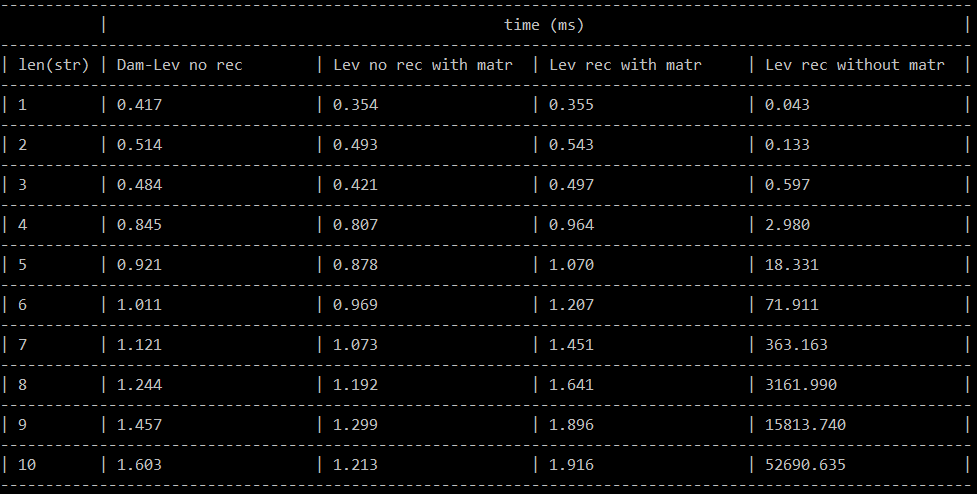
\includegraphics[scale=0.7]{test1.png}
            \caption{Результаты замера времени на строках длиной от 0 до 4}
            \label{png:test:1}
        
            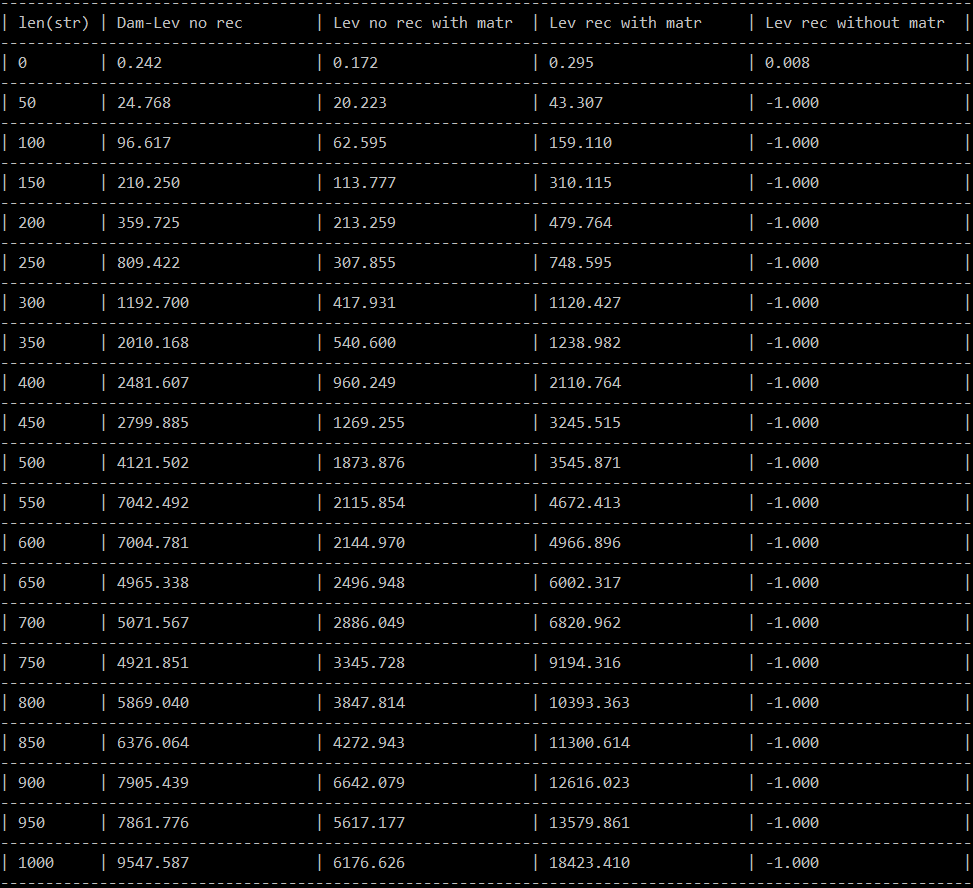
\includegraphics[scale=0.7]{test2.png}
            \caption{Результаты замера времени на строках длиной от 0 до 1000}
            \label{png:test:2}
        \end{figure}
    
        \begin{figure}[h!]
            \centering
            \begin{tikzpicture}
                \begin{axis}[
                    legend pos = north west,
                    ymin = 0,
                    grid = major,
                    xlabel = Длина слова,
                    ylabel = Время ms,
                    height = 0.5\paperheight, 
                    width = 0.75\paperwidth
                ]
                
                \addplot table[x=n,y=levrec] {data/test1.dat};
                \addplot table[x=n,y=levmatr] {data/test1.dat};
                \addplot table[x=n,y=levrecmatr] {data/test1.dat};
                \addplot table[x=n,y=damlev] {data/test1.dat};
                \legend{
                    р. Левенштейна рекурсивный без заполнения матрицы,
                    р. Левенштейна не рекурсивный,
                    р. Левенштейна рекурсивный с заполнением матрицы,
                    р. Дамерау-Левенштейна не рекурсивный
                };
                \end{axis}
            \end{tikzpicture}
            \caption{График зависимости времени работы алгоритмов от длин строк} 
            \label{graph:test:1}
        \end{figure}


        \begin{figure}[h!]
            \centering
            \begin{tikzpicture}
                \begin{axis}[
                    legend pos = north west,
                    xmin = 0,
                    ymin = 0,
                    grid = major,
                    xlabel = Длина слова,
                    ylabel = Время ms,
                    height = 0.5\paperheight, 
                    width = 0.75\paperwidth
                ]
                
                \addplot table[x=n,y=levmatr] {data/test2.dat};
                \addplot table[x=n,y=levrecmatr] {data/test2.dat};
                \addplot table[x=n,y=damlev] {data/test2.dat};
                \legend{
                    р. Левенштейна не рекурсивный,
                    р. Левенштейна рекурсивный с заполнением матрицы,
                    р. Дамерау-Левенштейна не рекурсивный
                };
                \end{axis}
            \end{tikzpicture}
            \caption{График зависимости времени работы алгоритмов от длин строк} 
            \label{graph:test:2}
        \end{figure}        

        % clear      10 peak cost: "71.0 Кб" heap "1.8 Кб" stacks
        % levmatr    10 peak cost: "71.0 Кб" heap "1.8 Кб" stacks
        % damlevmatr 10 peak cost: "71.0 Кб" heap "1.8 Кб" stacks
        % levrec     10 peak cost: "71.0 Кб" heap "1.8 Кб" stacks
        % levrecmatr 10 peak cost: "72.1 Кб" heap "2.2 Кб" stacks
        % 
        % clear      1000 peak cost: "73.0 Кб" heap "512 б" stacks
        % damlevmatr 1000 peak cost: "7.7 Мб" heap  "512 б" stacks
        % levmatr    1000 peak cost: "7.7 Мб" heap  "512 б" stacks
        % levrecmatr 1000 peak cost: "7.7 Мб" heap  "187.8 Кб" stacks

    \section{Вывод}
        В данном разделе были поставлены эксперименты по замеру времени
        выполнения каждого из алгоритмов. По итогам замеров не рекурсивный 
        алгоритм нахождения расстояния Левенштейна оказался самым быстродействующим
        на длинах строк превышающих 3 на 136 \% быстрее, чем алгоритм поиска
        расстояния Левенштейна рекурсивно с заполнением матрицы и на 42 \%,
        чем реализация алгоритм поиска расстояния Дамерау-Левенштейна. На строках
        длиной менее 3х символов рекурсивная реализиция выигрывает матричные, так
        как не выделяет в куче место под хранение матрицы.  
        
        По расходу памяти матричные алгоритмы проигрывают рекурсивному, так как
        максимальный размер используемой памяти имеет квадратичную ассимптотику
        (произведение длин строк), в то время как у рекурсивного - линейная (сумма длин строк).


\newpage